% ======================================================================
\section{Applications: From the List to Tests}\label{sec:applications}

\subsection{How each application was adapted}\label{subsec:adapt}
For every item on the application list we asked four questions, in this order. The answers are
collected in Table~\ref{tab:apps}.
\begin{enumerate}[leftmargin=1.5em,itemsep=1pt]
\item \emph{Which operator, and why is it wide?} Write the forward map and identify the mechanism
that gives fewer equations than unknowns: undersampling, decimation, a ``valid'' boundary, or a
bandwidth larger than the number of samples.
\item \emph{Is it HSS in the given coordinates?} Smooth or compactly supported kernels on a line
are, with ordered points. Oscillatory operators (Fourier, generic Toeplitz) are not. Their
off-diagonal ranks grow with block size (Table~\ref{tab:e1}: rank 512 for a $1024\times2048$
Toeplitz matrix).
\item \emph{If not, is there a \emph{unitary} transform to HSS form?} Unitary is essential.
By Lemma~\ref{lem:twosided} a unitary change of variables maps minimum-norm solutions to
minimum-norm solutions, so the solver can be applied to the transformed system unchanged. The
displacement-structure transforms the repo already uses (Toeplitz and Vandermonde to
Cauchy-like, via DFTs and unit-modulus diagonal scalings~\cite{gko}) are of exactly this type. A
non-unitary transform would change which solution is ``minimum-norm.''
\item \emph{Does the regularizer or weight stay simple in the solver's coordinates?} A
diagonal (leaf-block) weight in the HSS coordinates is cheap (memo~2). A weight that is diagonal in
the \emph{other} domain becomes circulant after the transform and is not covered.
\end{enumerate}
The fourth question decided where several applications land. The same NUDFT matrix serves seismic
interpolation and non-Cartesian MRI, but the HSS coordinates are physical space in one and
Cartesian $k$-space in the other. So spectral weights are cheap for MRI and expensive for MWNI.

\begin{table}[!htb]
\centering\footnotesize
\setlength{\tabcolsep}{3pt}
\begin{tabular}{@{}>{\raggedright\arraybackslash}p{2.2cm}>{\raggedright\arraybackslash}p{4.3cm}>{\raggedright\arraybackslash}p{3.2cm}>{\raggedright\arraybackslash}p{4.1cm}>{\raggedright\arraybackslash}p{1.6cm}@{}}
\toprule
application & operator, why wide & HSS form & meaning of $H^+b$ / weights & test\\
\midrule
non-uniform FFT, band-limited signals & $A_{jk}=e^{2\pi ikx_j}$, $m$ samples $<N$ coefficients & not HSS; $C=AF^*$ is Cauchy-like and HSS (F5) & minimum-energy band-limited interpolant & A1, Fig.~\ref{fig:a1}\\
seismic trace regularization & same $A$; $x_j$ = irregular trace positions, $N$ = regular grid & F5; columns = regular \emph{spatial} grid & min-norm Fourier reconstruction; MWNI spectral weights become circulant: not leaf-diagonal & A1 (+ memo 2)\\
non-Cartesian MRI (1-D) & $A_{jt}=e^{-2\pi i\xi_jt}$, $m$ $k$-space samples $<N$ pixels & F5 with roles swapped; columns = Cartesian $k$-space & $k$-space (spectral-prior) weights are diagonal: in scope; image-domain sparsity is not & memo 2\\
convolution, toy 1-D & ``valid'' or decimated convolution, $m\approx n/s$ & banded, exactly HSS (F4) & projection of the truth onto $\operatorname{Range}(H^*)$ & A2, Fig.~\ref{fig:a2}\\
deblurring / deconvolution & same; noisy data & F4 & min-norm amplifies noise ($\times7000$ at $\kappa=3.6\times10^4$) $\Rightarrow$ Tikhonov & A2 + memo 2\\
generic Toeplitz (inverse of Toeplitz) & random or non-smooth kernel, $m\times2m$ & not HSS (rank 512 at $n=2048$); $C=F_mTD^*F_n^*$ is (F6) & unitary $\Rightarrow$ min-norm preserved; $x=D^*F_n^*y$ & A3, Fig.~\ref{fig:a34}\\
ADMM / Douglas--Rachford & repeated projections onto $\{Hx=b\}$ & any of the above & each step needs $H^+(b-Hv)$: factor once & memo 2\\
basis pursuit & $\min\|x\|_1$ s.t.\ $Hx=b$ & F4 (seismic spikes) & IRLS inner loop = diagonal-weight min-norm & memo 2\\
higher dimensions & 2-D blur, decimated & HSS ranks grow like $\sqrt N$ & solver still exact; cost grows & A4, Fig.~\ref{fig:a34}\\
\bottomrule
\end{tabular}
\caption{The application list mapped to tests.}
\label{tab:apps}
\end{table}

\subsection{A1: band-limited interpolation from nonuniform samples}\label{subsec:a1}
Signal: $f(x)=\sum_{k=-512}^{511}c_ke^{2\pi ikx}$, real, with $|c_k|\propto(1+|k|/40)^{-3/2}$
(random phases). Data: $m=716$ jittered samples, plus a second case where the samples in
$[0.42,0.52]$ are removed (missing traces). The minimum-norm interpolant (Figure~\ref{fig:a1}a)
reproduces every sample to $10^{-11}$ and has $\|c_{\rm mn}\|=6.89<\|c\|=7.54$. Inside the gap it decays
to nearly zero. That is what ``minimum energy'' means: the solver adds no energy that the data do
not require. It is the classical behaviour that motivates weighted (MWNI-type) reconstruction.

\emph{Finding about the tree.} \texttt{hss\_constructor.m} splits row and column \emph{indices} in
half, independent of geometry. With jittered samples the halves cover the same intervals, and the
ranks of the index tree and a geometry-aligned tree agree (33/33). With a gap, the row halves drift
away from the column halves. Row clusters then interact with columns that are geometrically
\emph{adjacent} but in a different cluster, and the maximum rank doubles to 65, against 32 for a tree
whose row cuts are placed at the column cut positions (Figure~\ref{fig:a1}b; \texttt{mp\_tree\_aligned}
builds that tree in MATLAB). The solve is exact either way (errors $3.5\times10^{-13}$ and
$1.9\times10^{-13}$). Only the cost changes, and for strongly nonuniform sampling the cut rule should be
geometric.

\begin{figure}[!htb]
\centering
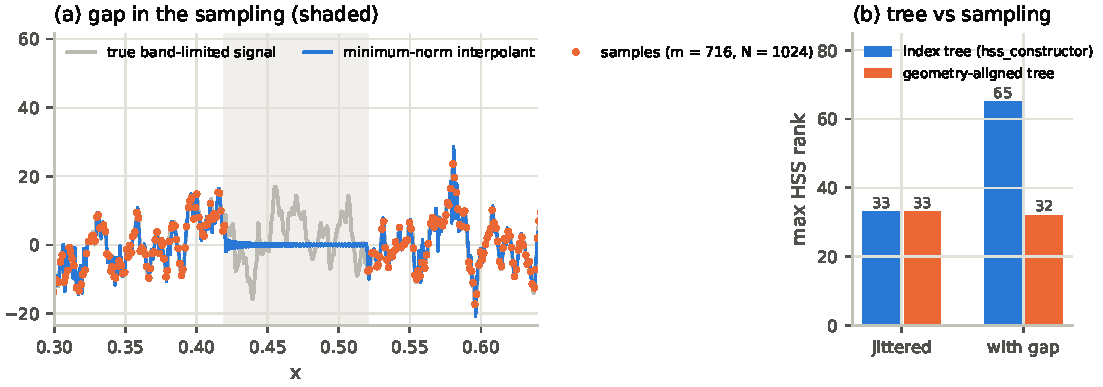
\includegraphics[width=\textwidth]{figures/m1_a1_nudft.pdf}
\caption{A1. (a) Minimum-norm band-limited interpolant with a 10\% gap ($N=1024$). (b) Maximum HSS
rank of $C=AF^*$ for the constructor's index-based tree and a geometry-aligned tree.}
\label{fig:a1}
\end{figure}

\subsection{A2: 1-D deconvolution}\label{subsec:a2}
Signal: the piecewise-smooth $x_0$ of Figure~\ref{fig:a2} ($n=2048$). Operator: Gaussian blur,
$\sigma=3$, stride 2, ``valid'' ($1012\times2048$, $\kappa=3.6\times10^4$, HSS rank 15, banded).
With exact data the computed $x$ agrees with the dense min-norm solution to $1.1\times10^{-12}$
($\approx\kappa u$) and is within 2.3\% of $x_0$. The minimum-norm solution is
$P_{\operatorname{Range}(H^*)}x_0$, and here $x_0$ is nearly in that range. With 0.1\% noise the
minimum-norm solution has relative error 7.3: it is the exact pseudo-inverse of noisy data. The solver
is not at fault; the problem needs regularization, which memo~2 provides.

\begin{figure}[!htb]
\centering
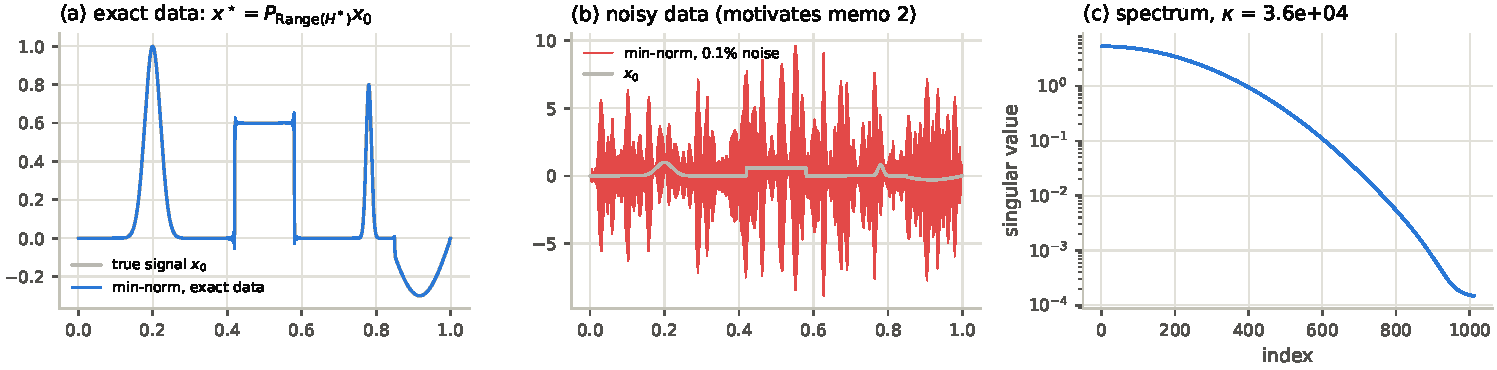
\includegraphics[width=\textwidth]{figures/m1_a2_deconv.pdf}
\caption{A2, decimated Gaussian deconvolution, exact and noisy data, and the spectrum of $H$.}
\label{fig:a2}
\end{figure}

\subsection{A3: generic Toeplitz through the Cauchy-like transform}\label{subsec:a3}
$T\in\mathbb{R}^{m\times 2m}$ random Toeplitz. $T$ itself has maximal HSS rank, $m/2$ at every size.
The Cauchy-like $C=F_mTD^*F_n^*$ has HSS rank 47 at $n=512$ and 97 at $n=65536$, growing by
$\approx7$ per doubling as the $\log n$ bound predicts~\cite{bt} (Figure~\ref{fig:a34}a,b). The whole pipeline
(FFT, $\mathcal M(C,F_mb)$, inverse FFT) matches the dense minimum-norm solution of $T$ to
$\le1.6\times10^{-12}$ (tolerance $10^{-12}$). Its imaginary part is $\le1.1\times10^{-12}$, as it must be
for real data. The cost is linear in $n$. Two practical notes. (i) The transform needs the two
node sets to stay separated: with $\theta=-1$ and $n=2m$ (or $m\mid n$) the nodes interlace
perfectly. For general $m,n$, $\min|\lambda_j-\mu_l|$ can be $O(1/(mn))$, and evaluating Cauchy-like
entries loses accuracy, so $\theta$ should be chosen from $\gcd(m,n)$. (ii) The ranks (up to 97)
exceed the blocksize-64 leaf slack. The legacy file would merge levels here; the current solver
does not.

\subsection{A4: higher dimensions}\label{subsec:a4}
Decimated (by 2 in each direction) Gaussian blur on an $n_1\times n_1$ image, $\sigma=1.5$\,px,
truncated at 5\,px, ordered lexicographically or along a Morton curve, compressed with the
constructor rule at tolerance $10^{-10}$. Figure~\ref{fig:a34}c: the maximum HSS rank grows like
$\sqrt N$, because an off-diagonal block couples the two halves of the image across an interface of
$O(n_1)$ pixels. Morton order lowers the constant but not the rate. The solver stays exact
(manufactured errors $\le10^{-14}$). The cost becomes $O(N^{3/2})$ (top-level ranks
$\sim\sqrt N$), so HSS is the wrong format past moderate 2-D sizes. For 2-D and 3-D the follow-up
is a format with strong admissibility or rank-adaptive skeletons ($\mathcal H^2$, HODLR with
recursive skeletonization). The minimum-norm reduction in this memo (unitary size reduction,
decoupling, forced solve) carries over block by block.

\begin{figure}[!htb]
\centering
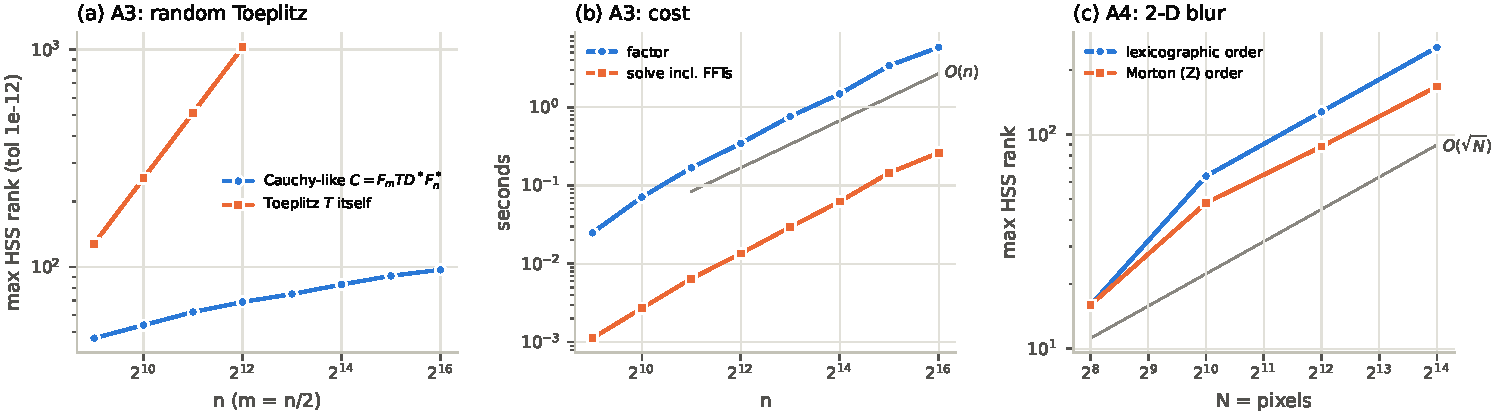
\includegraphics[width=\textwidth]{figures/m1_a3_a4.pdf}
\caption{A3 (a, b): random Toeplitz, HSS ranks before and after the unitary Cauchy-like transform,
and cost. A4 (c): rank growth for a 2-D blur.}
\label{fig:a34}
\end{figure}
